\documentclass[12pt,twoside]{article}
\usepackage[dvipsnames]{xcolor}
\usepackage{tikz,graphicx,amsmath,amsfonts,amscd,amssymb,bm,cite,epsfig,epsf,url}
\usepackage[hang,flushmargin]{footmisc}
\usepackage[colorlinks=true,urlcolor=blue,citecolor=blue]{hyperref}
\usepackage{amsthm,multirow,wasysym,appendix}
\usepackage{array,subcaption} 
% \usepackage[small,bf]{caption}
\usepackage{bbm}
\usepackage{pgfplots}
\usetikzlibrary{spy}
\usepgfplotslibrary{external}
\usepgfplotslibrary{fillbetween}
\usetikzlibrary{arrows,automata}
\usepackage{thmtools}
\usepackage{blkarray} 
\usepackage{textcomp}
\usepackage[left=0.8in,right=1.0in,top=1.0in,bottom=1.0in]{geometry}
\usepackage{pifont}
\usepackage{tikz-qtree}

%% Probability operators and functions
%
% \def \P{\mathrm{P}}
\def \P{\mathrm{P}}
\def \E{\mathrm{E}}
\def \Var{\mathrm{Var}}
\let\var\Var
\def \Cov {\mathrm{Cov}} \let\cov\Cov
\def \MSE {\mathrm{MSE}} \let\mse\MSE
\def \sgn {\mathrm{sgn}}
\def \R {\mathbb{R}}
\def \C {\mathbb{C}}
\def \N {\mathbb{N}}
\def \Z {\mathbb{Z}}
\def \cV {\mathcal{V}}
\def \cS {\mathcal{S}}

\newcommand{\RR}{\ensuremath{\mathbb{R}}}

\DeclareMathOperator*{\argmin}{arg\,min}
\DeclareMathOperator*{\argmax}{arg\,max}
\newcommand{\red}[1]{\textcolor{red}{#1}}
\newcommand{\blue}[1]{\textcolor{blue}{#1}}
\newcommand{\green}[1]{\textcolor{ForestGreen}{ #1}}
\newcommand{\fuchsia}[1]{\textcolor{RoyalPurple}{ #1}}



%
%% Probability distributions
%
%\def \Bern    {\mathrm{Bern}}
%\def \Binom   {\mathrm{Binom}}
%\def \Exp     {\mathrm{Exp}}
%\def \Geom    {\mathrm{Geom}}
% \def \Norm    {\mathcal{N}}
%\def \Poisson {\mathrm{Poisson}}
%\def \Unif    {\mathrm {U}}
%
\DeclareMathOperator{\Norm}{\mathcal{N}}

\newcommand{\bdb}[1]{\textcolor{red}{#1}}

\newcommand{\ml}[1]{\mathcal{ #1 } }
\newcommand{\wh}[1]{\widehat{ #1 } }
\newcommand{\wt}[1]{\widetilde{ #1 } }
\newcommand{\conj}[1]{\overline{ #1 } }
\newcommand{\rnd}[1]{\tilde{ #1 } }
\newcommand{\rv}[1]{ \rnd{ #1}  }
\newcommand{\rM}{\rnd{ m}  }
\newcommand{\rx}{\rnd{ x}  }
\newcommand{\ry}{\rnd{ y}  }
\newcommand{\rz}{\rnd{ z}  }
\newcommand{\ra}{\rnd{ a}  }
\newcommand{\rb}{\rnd{ b}  }
\newcommand{\rt}{\rnd{ t}  }
\newcommand{\rs}{\rnd{ s}  }


\newcommand{\rpc}{\widetilde{ pc}  }
\newcommand{\rndvec}[1]{\vec{\rnd{#1}}}

\def \cnd {\, | \,}
\def \Id { I }
\def \J {\mathbf{1}\mathbf{1}^T}

\newcommand{\op}[1]{\operatorname{#1}}
\newcommand{\setdef}[2]{ := \keys{ #1 \; | \; #2 } }
\newcommand{\set}[2]{ \keys{ #1 \; | \; #2 } }
\newcommand{\sign}[1]{\op{sign}\left( #1 \right) }
\newcommand{\trace}[1]{\op{tr}\left( #1 \right) }
\newcommand{\tr}[1]{\op{tr}\left( #1 \right) }
\newcommand{\inv}[1]{\left( #1 \right)^{-1} }
\newcommand{\abs}[1]{\left| #1 \right|}
\newcommand{\sabs}[1]{| #1 |}
\newcommand{\keys}[1]{\left\{ #1 \right\}}
\newcommand{\sqbr}[1]{\left[ #1 \right]}
\newcommand{\sbrac}[1]{ ( #1 ) }
\newcommand{\brac}[1]{\left( #1 \right) }
\newcommand{\bbrac}[1]{\big( #1 \big) }
\newcommand{\Bbrac}[1]{\Big( #1 \Big)}
\newcommand{\BBbrac}[1]{\BIG( #1 \Big)}
\newcommand{\MAT}[1]{\begin{bmatrix} #1 \end{bmatrix}}
\newcommand{\sMAT}[1]{\left(\begin{smallmatrix} #1 \end{smallmatrix}\right)}
\newcommand{\sMATn}[1]{\begin{smallmatrix} #1 \end{smallmatrix}}
\newcommand{\PROD}[2]{\left \langle #1, #2\right \rangle}
\newcommand{\PRODs}[2]{\langle #1, #2 \rangle}
\newcommand{\der}[2]{\frac{\text{d}#2}{\text{d}#1}}
\newcommand{\pder}[2]{\frac{\partial#2}{\partial#1}}
\newcommand{\derTwo}[2]{\frac{\text{d}^2#2}{\text{d}#1^2}}
\newcommand{\ceil}[1]{\lceil #1 \rceil}
\newcommand{\Imag}[1]{\op{Im}\brac{ #1 }}
\newcommand{\Real}[1]{\op{Re}\brac{ #1 }}
\newcommand{\norm}[1]{\left|\left| #1 \right|\right| }
\newcommand{\norms}[1]{ \| #1 \|  }
\newcommand{\normProd}[1]{\left|\left| #1 \right|\right| _{\PROD{\cdot}{\cdot}} }
\newcommand{\normTwo}[1]{\left|\left| #1 \right|\right| _{2} }
\newcommand{\normTwos}[1]{ \| #1  \| _{2} }
\newcommand{\normZero}[1]{\left|\left| #1 \right|\right| _{0} }
\newcommand{\normTV}[1]{\left|\left| #1 \right|\right|  _{ \op{TV}  } }% _{\op{c} \ell_1} }
\newcommand{\normOne}[1]{\left|\left| #1 \right|\right| _{1} }
\newcommand{\normOnes}[1]{\| #1 \| _{1} }
\newcommand{\normOneTwo}[1]{\left|\left| #1 \right|\right| _{1,2} }
\newcommand{\normF}[1]{\left|\left| #1 \right|\right| _{\op{F}} }
\newcommand{\normLTwo}[1]{\left|\left| #1 \right|\right| _{\ml{L}_2} }
\newcommand{\normNuc}[1]{\left|\left| #1 \right|\right| _{\ast} }
\newcommand{\normOp}[1]{\left|\left| #1 \right|\right|  }
\newcommand{\normInf}[1]{\left|\left| #1 \right|\right| _{\infty}  }
\newcommand{\proj}[1]{\mathcal{P}_{#1} \, }
\newcommand{\diff}[1]{ \, \text{d}#1 }
\newcommand{\vc}[1]{\boldsymbol{\vec{#1}}}
\newcommand{\rc}[1]{\boldsymbol{#1}}
\newcommand{\vx}{\vec{x}}
\newcommand{\vy}{\vec{y}}
\newcommand{\vz}{\vec{z}}
\newcommand{\vu}{\vec{u}}
\newcommand{\vv}{\vec{v}}
\newcommand{\vb}{\vec{\beta}}
\newcommand{\va}{\vec{\alpha}}
\newcommand{\vaa}{\vec{a}}
\newcommand{\vbb}{\vec{b}}
\newcommand{\vg}{\vec{g}}
\newcommand{\vw}{\vec{w}}
\newcommand{\vh}{\vec{h}}
\newcommand{\vbeta}{\vec{\beta}}
\newcommand{\valpha}{\vec{\alpha}}
\newcommand{\vgamma}{\vec{\gamma}}
\newcommand{\veta}{\vec{\eta}}
\newcommand{\vnu}{\vec{\nu}}
\newcommand{\rw}{\rnd{w}}
\newcommand{\rvnu}{\vc{\nu}}
\newcommand{\rvv}{\rndvec{v}}
\newcommand{\rvw}{\rndvec{w}}
\newcommand{\rvx}{\rndvec{x}}
\newcommand{\rvy}{\rndvec{y}}
\newcommand{\rvz}{\rndvec{z}}
\newcommand{\rvX}{\rndvec{X}}


\newtheorem{theorem}{Theorem}[section]
% \declaretheorem[style=plain,qed=$\square$]{theorem}
\newtheorem{corollary}[theorem]{Corollary}
\newtheorem{definition}[theorem]{Definition}
\newtheorem{lemma}[theorem]{Lemma}
\newtheorem{remark}[theorem]{Remark}
\newtheorem{algorithm}[theorem]{Algorithm}

% \theoremstyle{definition}
%\newtheorem{example}[proof]{Example}
\declaretheorem[style=definition,qed=$\triangle$,sibling=definition]{example}
\declaretheorem[style=definition,qed=$\bigcirc$,sibling=definition]{application}

%
%% Typographic tweaks and miscellaneous
%\newcommand{\sfrac}[2]{\mbox{\small$\displaystyle\frac{#1}{#2}$}}
%\newcommand{\suchthat}{\kern0.1em{:}\kern0.3em}
%\newcommand{\qqquad}{\kern3em}
%\newcommand{\cond}{\,|\,}
%\def\Matlab{\textsc{Matlab}}
%\newcommand{\displayskip}[1]{\abovedisplayskip #1\belowdisplayskip #1}
%\newcommand{\term}[1]{\emph{#1}}
%\renewcommand{\implies}{\;\Rightarrow\;}



\begin{document}

\begin{center}
{\large{\textbf{Homework 12}} } \vspace{0.2cm}\\
Due May 7 at 11 pm
\\
\end{center}
Unless stated otherwise, justify any answers you give.
You can work in groups, but each
student must write their own solution based on their own
understanding of the problem.

When uploading your homework to Gradescope you will have to
select the relevant pages for each question.  Please submit each
problem on a separate page (i.e., 1a and~1b can be on the same page but 1
and 2 must be on different pages).  We understand that this may be
cumbersome but this is the best way for the grading team to grade your
homework assignments and provide feedback in a timely manner.  Failure
to adhere to these guidelines may result in a loss of points.
Note that it may take some time to
select the pages for your submission.  Please plan accordingly.  We
suggest uploading your assignment at least 30 minutes before the deadline
so you will have ample time to select the correct pages for your
submission.  If you are using \LaTeX, consider using the minted or
listings packages for typesetting code.  
\\

\begin{enumerate}

 \item (Augmented dataset) Ridge regression is equivalent to applying OLS on an expanded dataset that has additional examples. Describe these additional examples in detail. Intuitively, what effect do these additional examples have?

 \begin{itemize}
     \color{blue}
     \item Ridge regression can more or less be though of as adding a number of examples with values that are far away from the mean of each feature, but doing so in a way such that there is no correlation between each feature. this raises the feature variance within our training set but not the covariance. this reduces the variance of our estimator in each direction, so it is more likely to be near the mean of each feature. 
     \item this intuitively can be thought of syntactically adding more high variance but uncorrelated examples to our training data which lowers the impact to observed training examples within our data.
     \end{itemize}

\item  (Correlated features) Consider a regression problem where the response only depends on one feature, but we don't know it, so we incorporate an additional feature into the model that happens to be very correlated with the first feature. More specifically, let $y \in \R^{n}$ be defined by
\begin{align}
y := \beta_{\op{prior}} x_1 + z, 
\end{align}
where $\beta_{\op{prior}} \in \R$ is the true coefficient, $x_1 \in \R^n$ is the first feature vector, and $z \in \R^{n}$ is additive noise. The second feature vector is given by $x_2\in \R^n$ and can be decomposed into
\begin{align}
x_2 = \alpha x_1 + \sqrt{1-\alpha^2} x_{\perp},
\end{align}  
where $x_{\perp}$ is orthogonal to $x_1$. The vectors $x_1$, $x_2$, $x_{\perp}$ and $z$ all have unit $\ell_2$ norm. In addition, we assume
\begin{align}
x_1^Tz = 0.1, \\
x_{\perp}^Tz = 0.1.
\end{align}
We fit a linear regression model to $y$ using the feature matrix 
  \begin{align}
  X & = \MAT{x_1^T \\ x_2^T}.
  \end{align} 
 \begin{enumerate}
  \item What does the OLS estimator of the coefficients $\beta_{\op{OLS}}$ equal to when $\alpha \rightarrow 1$? Explain what is happening. \\
\emph{Hint:} Use the fact that for any $a$, $b$, $c$, and $d$ such that $ad \neq bc$
\begin{align}
 \MAT{a & b \\ c & d}^{-1} = \frac{1}{ad-bc} \MAT{d & -b \\ -c & a}.
\end{align}
\begin{itemize}
\color{red}
    \item The OLS estimator is given by $\beta_{OLS} = (\Sigma_{X})^{-1} \Sigma_{x,y}$
    \item When $\alpha \rightarrow 1$, $x_2$ becomes collinear with $x_1$. 
    \item where the feature matrix $X$ becomes rank deficient such that $det(\Sigma_{x}) \rightarrow 0$ and thus $(\Sigma_{x})^{-1}$ is not well-defined, which leading to unreliable estimates of the model parameter $\beta$
\end{itemize}
   \item  What does the corresponding estimate of the response $y_{\op{OLS}} := X^T\beta_{\op{OLS}}$ equal to when $\alpha \rightarrow 1$? Is it collinear with the true feature $x_1$ when $\alpha \rightarrow 1$? Explain what is happening.
\begin{itemize}
    \color{blue}
    \item our prediction $y_{OLS} := X^T \beta_{OLS}$ remains accurate
    \item this is because the features of $X, (x_1,x_2)$ are collinear but capture the linear relationship with respect to the response $y_{OLS}$
    \item However, our prediction $y_{OLS}$ does not necessarily have to be co-linear with $X_1$ since the estimate is based on both $x_1,x_2$
\end{itemize}
   
  \item What does the ridge regression estimator of the coefficients $\beta_{\op{RR}}$ equal to when $\alpha \rightarrow 1$ and the regularization parameter $\lambda >0$ is fixed? Describe the difference with the OLS estimate.
\begin{itemize}
   \color{purple}
    \item the closed for solution for ridge regression is given by $$\beta{rr}=(\Sigma_{x}+\lambda I)^{-1}X^Ty$$
\item as $\alpha \rightarrow 1$ $x_2$ becomes collinear with $x_!$ however$ (\Sigma_{x}+\lambda I)$ remains inevitable. 
\itme This differs from the OLS estimate which is not guaranteed to be inevitable, and thus ridge regression provides much more stable estimates of $\beta$
\end{itemize}

  
  \item  What does the corresponding estimate of the response $y_{\op{RR}} := X^T\beta_{\op{RR}}$ equal to when $\alpha \rightarrow 1$? Is it collinear with the true feature $x_1$?

  \begin{itemize}
      \color{orange}
      \item as $\alpha \rightarrow 1$, the estimate of the response  is given by $$y_{rr} = X^T \beta_{rr}$$. This estimate is not necessarily colinear with $x_1$, because our prediction is based on both $x_1$ and $x_2$.
  \end{itemize}
  \end{enumerate} 
  
 \item (Prior knowledge) Consider a linear regression problem where we have prior information indicating that the coefficients should be close to a certain value $\beta_{\op{prior}}$. 
 \begin{enumerate}
   \item How can you incorporate this prior knowledge if you are using ridge regression? Write the corresponding optimization problem. 
   \begin{itemize}
       \color{red}
       \item there are two potential ways. 
       \item firstly we could simply write or loss function as $$\ell(\beta)=||y-X^t\beta||_{2}^{2}+\lambda||\beta_{prior}-\beta||_{2}^2$$
       \item so our optimization would be $$argmin_{\beta\in\mathbb{R}^p}||y-X^t\beta||_{2}^{2}+\lambda||\beta_{prior}-\beta||_{2}^2$$
       \item this approach is equivalent to penalizing for the distance of it's parameters in $\ell_2$ space for $\beta_{prior}$
   \end{itemize}

   
   \begin{itemize}
   
       \color{blue}
       \item another valiid aproach could be modeling this as a baysian problem 
       \item yes you can, and doing so makes this a Bayesian modeling question
       \item we know that suppose we have dataset $\mathcal{D}$ we know that $$P(\beta|\mathcal{D})=\frac{P(\mathcal{D}|\beta)P(\beta)}{P(\beta, \mathcal{D})}\propto P(\mathcal{D}|\beta)P(\beta) = \mathcal{L}_{\beta}(\mathcal{D})P(\beta)$$
       \item so our goal is to find $\beta^{*}=argmax_{\beta\in \mathbb{R}}P(\mathcal{D}|\beta)P(\beta)$
   \end{itemize}
   \item Assume that the data are generated according to a linear model $\rnd{y}:= X^T \beta_{\op{t}} + \rnd{z}$, where $\beta_{ture}\in \R^{p}$ and $X  \in \R^{p \times n}$ are fixed and the entries of $\rnd{z}$ are i.i.d. with zero mean and variance $\sigma^2$. Does the modification change the mean or the covariance matrix of the coefficient estimate with respect to the ridge-regression estimator? If so, report the new value.
   \begin{itemize}

\color{blue}
\item the blue section is kind of an aside . 
\item we can reconcile the two baysian and optimization view points with this new information and assuming $\beta\sim \mathcal{N}(\beta_{prior}, \lambda ^2)$
\item given $\Tilde{z}\sim \mathcal{N}(0,\sigma^2)$ we can see that $E[\hat{y}]=E[X^T\beta+\Tilde{z}]=beta^tx$
\item as we well as $var(\hat{y})=var(X^T\beta+\Tilde{z})=\Sigma^2$
\item thus we have $P(y|x,\beta)=\hat{\Tilde{y}}\sim \mathcal{N}(\beta^tx, \sigma^2)$
       \item now we want to try the likelihood of our dataset given $\beta$ 
       $$\mathcal{L}_{\beta}(\mathcal{D})=\Pi_{i=1}^{n}P(y_i|x_i,\beta)$$ we are going to take the arg max so we can look at the log likelihood 
$$\ell=\Sigma_{i=1}^{n}log(P(y_i|x_i,\beta))=\Sigma_{i=1}^{N}log(\frac{1}{\sqrt{2\pi}\sigma}e^{\frac{(y_i-\beta x_i)^2}{2\sigma ^2}})={N}(log(\frac{1}{\sqrt{2\pi}\sigma})-\frac{1}{2\sigma^2}\Sigma_{i=1}^{n}{(y_i-\beta x_i)^2})
$$ $$\propto-\frac{1}{2\sigma^2}\Sigma_{i=1}^{n}{(y_i-\beta x_i)^2}=-\frac{1}{2\sigma^2}||y-X^t\beta||_{2}^{2}$$ 
\item so our overall estimate is given as $$\beta^{*}=argmax_{\beta\in \mathbb{R}}P(\mathcal{D}|\beta)P(\beta)=-\frac{1}{2\sigma^2}|y-X^t\beta|_{2}^{2}P(\beta)$$
assume $\beta\sim \mathcal{N}(\beta_{prior}, \lambda^2)$ if this is the case we can write $$log(P(\beta))=log(\frac{1}{\sqrt{2\pi}\lambda}e^{-\frac{1}{2}(\frac{\beta-\beta_{prior}}{\lambda})^2})=log(\frac{1}{\sqrt{2\pi}\lambda})-\frac{1}{2\lambda^2}||\beta-\beta_{prior}||_{2}^{2}\propto-\frac{1}{2\lambda^2}||\beta-\beta_{prior}||_{2}^{2}$$ 
\item notice that we can express this as $$\beta^{*}=argmax_{\beta\in \mathbb{R}}P(\mathcal{D}|\beta)P(\beta)=argmax_{\beta\in \mathbb{R}}log(P(\mathcal{D}|\beta)P(\beta))$$$$= argmax_{\beta\in \mathbb{R}}log(P(\mathcal{D}|\beta))+log(P(\beta))=argmax_{\beta\in \mathbb{R}}-\frac{1}{2\sigma^2}||y-X^t\beta||_{2}^{2}-\frac{1}{2\lambda^2}||\beta-\beta_{prior}||_{2}^{2}$$$$=argmax_{\beta}-\frac{1}{2\sigma^2}||y-X^t\beta||_{2}^{2}-\frac{1}{2\lambda^2}||\beta-\beta_{prior}||_{2}^{2}=argmax_{\beta}-||y-X^t\beta||_{2}^{2}-\frac{1}{\lambda}||\beta-\beta_{prior}||_{2}^{2}$$ $$=argmin_{\beta}||y-X^t\beta||_{2}^{2}+\frac{1}{\lambda}||\beta-\beta_{prior}||_{2}^{2}=argmax_{\beta}||y-X^t\beta||_{2}^{2}+{\lambda}||\beta-\beta_{prior}||_{2}^{2}$$
\end{itemize}
   
   \begin{itemize}
       \color{red}
       \item  given we can write  $$\beta^{*}=argmin_{\beta\in\mathbb{R}^p}||y-X^t\beta||_{2}^{2}+\lambda||\beta_{prior}-\beta||_{2}^2$$
       \item we optimize this question $$\frac{\partial \ell}{\partial \beta}=\frac{\partial }{\partial \beta}(yy^T -2X^T\beta Y+ X^T\beta \beta^T X + \lambda(\beta_{prior}^2 -2\beta_{prior}\beta+\beta \beta^t)$$ $$=-2X^TY +2X^t\beta X-2\lambda \beta_{prior}+2\lambda \beta$$
       \item we can know check the Hessian $$\frac{\partial }{\partial \beta}(-2X^TY 2X^t\beta X-2\lambda \beta_{prior}+\lambda 2\beta)=2X^TX+2\lambda =2\Sigma_{X}+2\lambda$$ and as we know covariance matrices are positive semi definite, we know the hessian is positive semi define and thus any extrema with the first order condition satisfied will be a global min of our loss function 
       \item we can get such a min by solving $$-2X^TY +2X^t\beta X-2\lambda \beta_{prior}+\lambda 2\beta=0\iff \beta^{*}=(\Sigma_{X}+\frac{\lambda }{n-1}I)^{-1}(\Sigma_{x,y}+\frac{\lambda \beta_{prior} }{n-1} I) $$
       
   \end{itemize}


\begin{itemize}
    \color{purple}
    \item so we finally have $$\beta^{*}=(\Sigma_{X}+\frac{\lambda }{n-1}I)^{-1}(\Sigma_{x,y}+\frac{\lambda \beta_{prior} }{n-1} I)=\beta_{rr}+(\Sigma_{X}+\frac{\lambda }{n-1}I)^{-1}(\frac{\lambda \beta_{prior} }{n-1} I) $$
    \item notice that this is just the ridge regression estimator plus the term of all random variables and thus constant $$(\Sigma_{X}+\frac{\lambda }{n-1}I)^{-1}(\frac{\lambda \beta_{prior} }{n-1} I)$$ and this term is independent $\Tilde{z}, \Tilde{y}, \Tilde{\beta}$ 
    \item $$E[\beta^{*}]=E[\beta_{rr}+(\Sigma_{X}+\frac{\lambda }{n-1}I)^{-1}(\frac{\lambda \beta_{prior} }{n-1} I)]=E[\beta_{rr}]+\beta_{prior}(\Sigma_{X}+\frac{\lambda }{n-1}I)^{-1}(\frac{\lambda }{n-1} I) $$ so we shift proportionally to the variance of our data, the strength of regularization, and our prior on $\beta$
    \item similarly our variance will be increased proportionally by $\beta_{\prior}$ and we will have variance  $\var(b_rr)+(\beta_{prior}(\Sigma_{X}+\frac{\lambda }{n-1}I)^{-1}(\frac{\lambda }{n-1} I))^2$

\end{itemize}
   
   \end{enumerate}

\item (Ridge and Lasso)
Using linear regression with OLS estimator, Ridge, and Lasso regularization, predict temperature in the \texttt{regression.ipynb} notebook. Try different regularization strength $\lambda \in \{10^{-5}, 10^{-4}, 10^{-3}, 10^{-2}, 10^{-1}, 1, 10, 100\}$ and numbers of training samples $n \in \{200, 600, 2000\}$ .

\begin{enumerate}
\item Plot the root mean squared errors for the training and validation sets. Identify the value of $\lambda$ that gives the lowest validation loss for each experiment.
\begin{itemize}
    \color{orange}
    \item here are my results 
    \begin{itemize}
         \item rmse for OLS train with 200 samples was archived at $\lambda=$0.1
\item lowest rmse for ridge train with 200 samples was 10

\item lowest rmse for lasso train with 200 samples was archived at $\lambda=$ 0.1

\item lowest rmse for ridge train with 200 samples was archived at $\lambda=$ 10

\item lowest rmse for lasso test with 200 samples was archived at $\lambda=$ at 1

\item lowest rmse for ridge test with 200 samples was archived at $\lambda=$ 100

 \item rmse for OLS train with 600 samples was archived at $\lambda=$ 1e-05

\item lowest rmse for ridge train with 600 samples was archived at $\lambda=$ at 10

\item lowest rmse for lasso train with 600 samples was archived at $\lambda=$ 1e-05

\item lowest rmse for ridge train with 600 samples was archived at $\lambda=$ 10

\item lowest rmse for lasso test with 600 samples was archived at $\lambda=$ at 1

\item lowest rmse for ridge test with 600 samples was archived at $\lambda=$ 100

 \item rmse for OLS train with 2000 samples was archived at $\lambda=$ 0.1

\item lowest rmse for ridge train with 2000 samples was archived at $\lambda=$ at 100

\item lowest rmse for lasso train with 2000 samples was archived at $\lambda=$ 0.1

\item lowest rmse for ridge train with 2000 samples was archived at $\lambda=$ 100

\item lowest rmse for lasso test with 2000 samples was archived at $\lambda=$ at 1

\item lowest rmse for ridge test with 2000 samples was archived at $\lambda=$ 100
\end{itemize}
\item here are my plots
\begin{itemize}
    \item 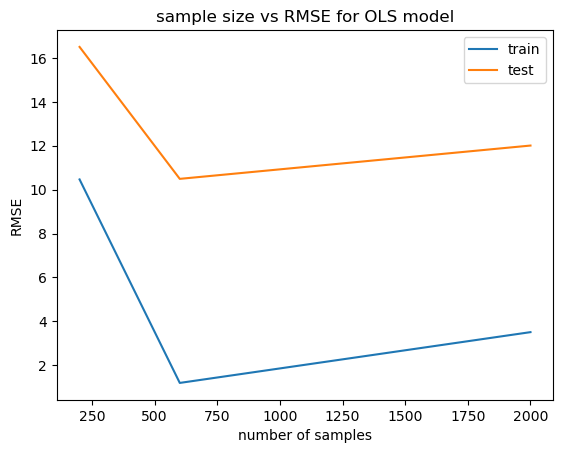
\includegraphics[width=10cm]{homework/homework_12/immages/hw_12_1.png}
        \item 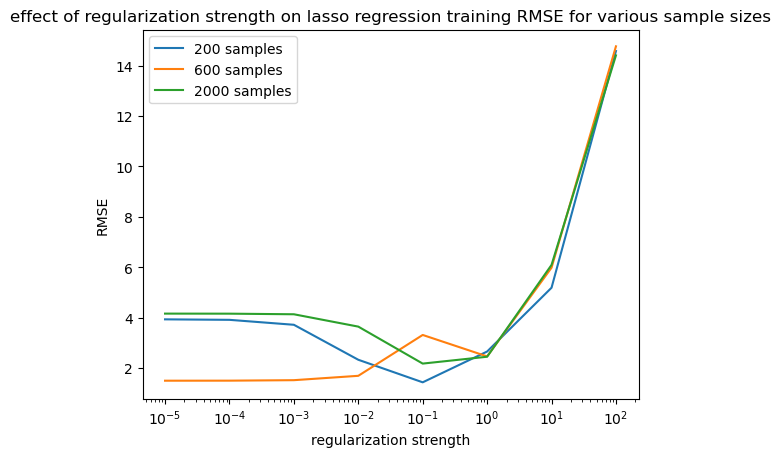
\includegraphics[width=10cm]{homework/homework_12/immages/hw_12_2.png}
            \item 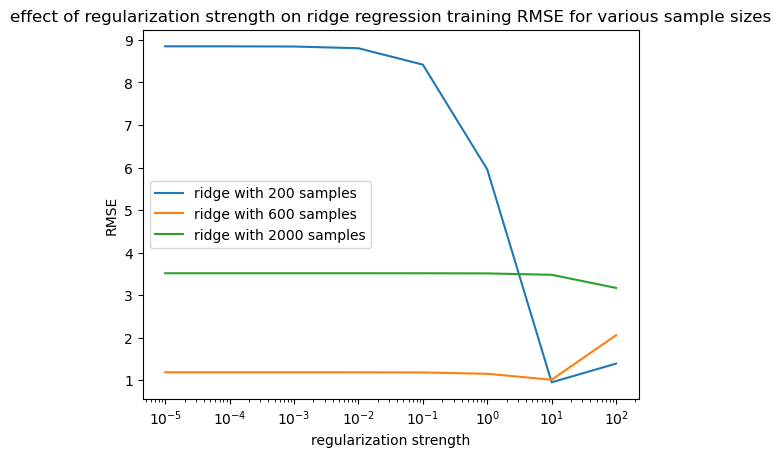
\includegraphics[width=10cm]{homework/homework_12/immages/hw_12_3.png}
                \item 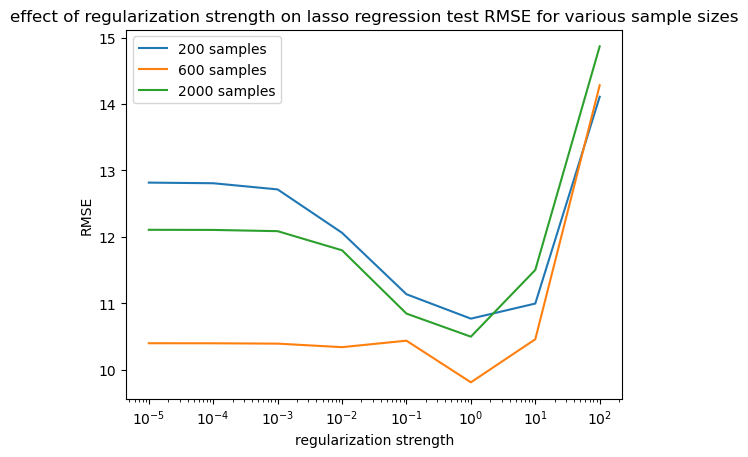
\includegraphics[width=10cm]{homework/homework_12/immages/hw_12_4.png}
                    \item 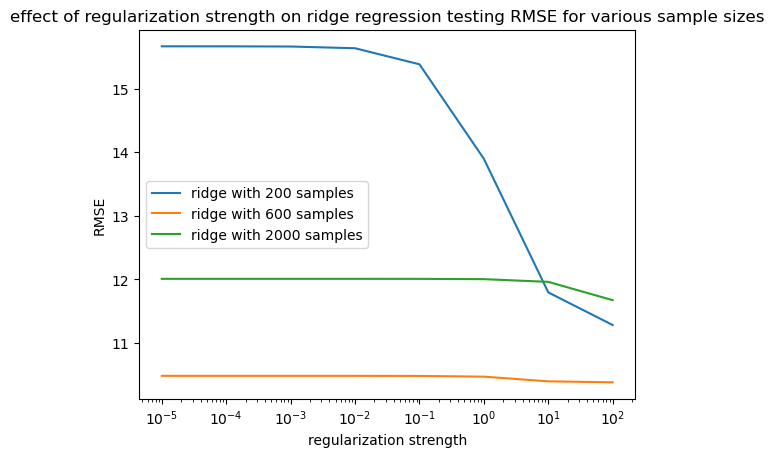
\includegraphics[width=10cm]{homework/homework_12/immages/hw_12_5.png}
\end{itemize}
\end{itemize}


\item Plot the coefficients of the best model for each setting. The feature names are stored in variable \textit{cities}. Report the five coefficients with the greatest magnitudes. Discuss the differences between OLS, Ridge, and Lasso regression.

\begin{itemize}
    \color{orange}
   
\item here are my plots
\begin{itemize}
    \item 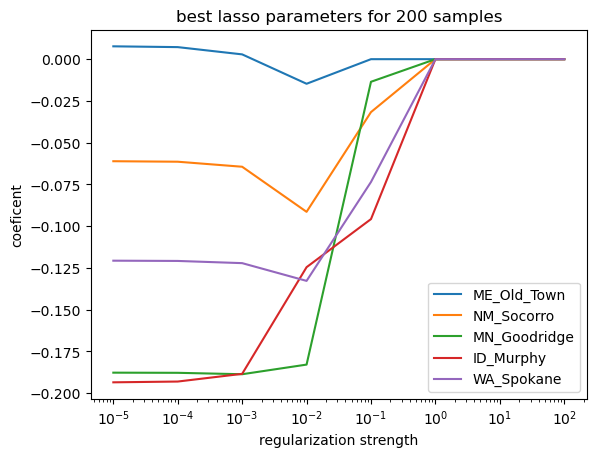
\includegraphics[width=10cm]{homework/homework_12/immages/hw_12_6.png}
        \item 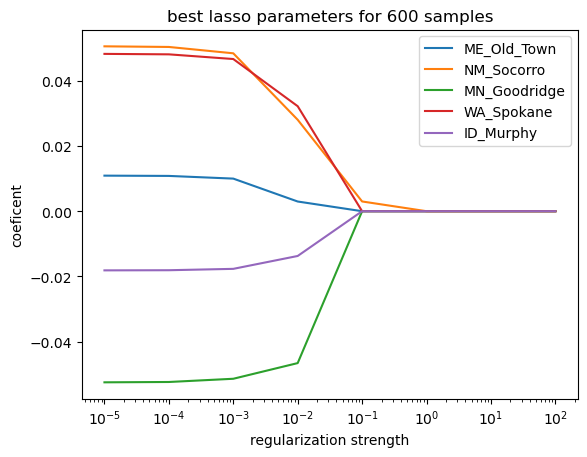
\includegraphics[width=10cm]{homework/homework_12/immages/hw_12_7.png}
            \\ 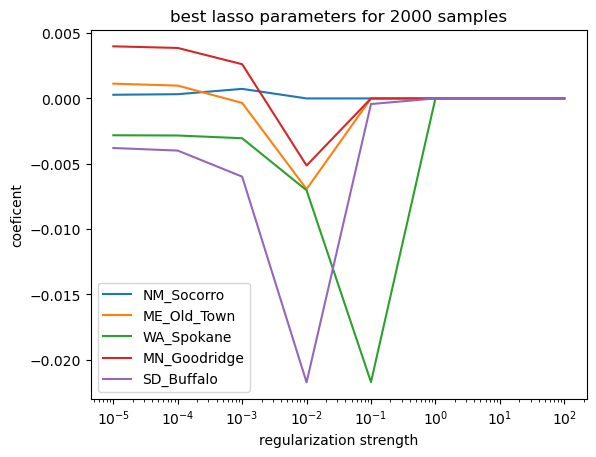
\includegraphics[width=10cm]{homework/homework_12/immages/hw_12_8.png}
        \\ 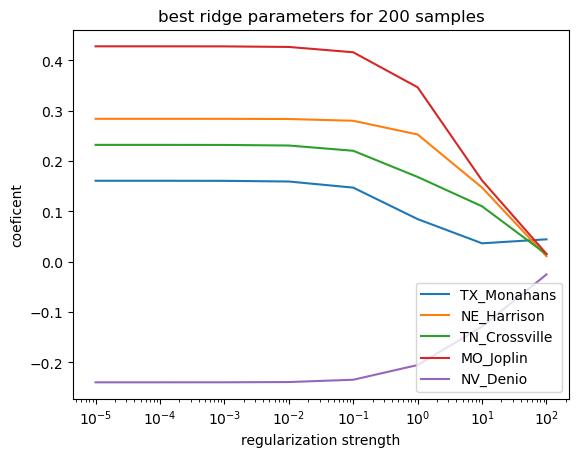
\includegraphics[width=10cm]{homework/homework_12/immages/hw_12_9.png}
            \\ 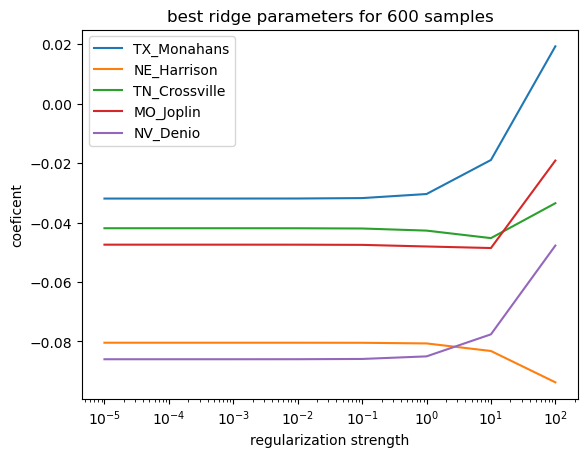
\includegraphics[width=10cm]{homework/homework_12/immages/hw_12_10.png}
        \\ 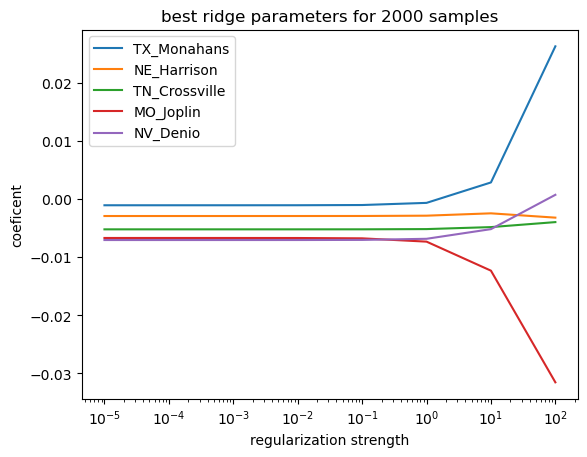
\includegraphics[width=10cm]{homework/homework_12/immages/hw_12_11.png}
\end{itemize}
\ITEM we can see from these plots that lasso regression will chose a spare solution that is will fully reduce some parameters to have a value of zero, while ridge regression on the other hand will reduce parameters to just be near zero .
 \end{itemize}
\end{enumerate}

\end{enumerate}
 
\end{document}
